\documentclass[12pt,letterpaper]{article}
\usepackage[utf8]{inputenc}
\usepackage[T1]{fontenc}
\usepackage{lmodern}
\IfFileExists{spanish.ldf}{\usepackage[spanish,es-tabla]{babel}}{\usepackage{babel}}
\usepackage[margin=2.54cm]{geometry}
\usepackage{microtype}
\usepackage{graphicx}
\usepackage{booktabs,tabularx,longtable,array}
\usepackage{float}
\usepackage{enumitem}
\usepackage{setspace}
\usepackage{xcolor}
\usepackage[authoryear,round]{natbib}
\usepackage{hyperref}
\usepackage{xurl}
\hypersetup{colorlinks=true,linkcolor=black,urlcolor=blue,citecolor=black,
  pdftitle={Sumativa 1: preparación reproducible de Compra Ágil},
  pdfauthor={Grupo 7 MCDI500}}
\renewcommand{\contentsname}{Índice}
\renewcommand{\refname}{Referencias}
\renewcommand{\figurename}{Figura}
\renewcommand{\tablename}{Tabla}
\renewcommand{\bibsection}{\section*{Referencias}\addcontentsline{toc}{section}{Referencias}}
\setlength{\bibhang}{1.27cm}
\setlength{\bibsep}{0.8\baselineskip}
\setlength{\parindent}{0pt}
\setlength{\parskip}{6pt}
\setlength{\emergencystretch}{3em}
\setlist{nosep,leftmargin=*}
\setstretch{1.15}
\newcolumntype{Y}{>{\raggedright\arraybackslash}X}
\newcommand{\archivo}[1]{\path{#1}}
% Generado por F2; no editar a mano.
\newcommand{\FilasOriginal}{11.177}
\newcommand{\ColumnasOriginal}{63}
\newcommand{\Ordenes}{541}
\newcommand{\Proveedores}{277}
\newcommand{\DuplicadosAdicionales}{6}
\newcommand{\OrdenesMultirrubro}{180}
\newcommand{\OrdenesConciliadas}{538}
\newcommand{\ExcepcionesDetalle}{3}
\newcommand{\NetoTotal}{669.016.915,21}
\newcommand{\ExtremosNeto}{61}
\newcommand{\UmbralNeto}{3.723.495,50}
\newcommand{\ExtremosMapa}{60}
\newcommand{\UmbralMapa}{4.379.267,38}
\newcommand{\TamanoDesconocido}{56}
\newcommand{\FechaMin}{2025-01-06}
\newcommand{\FechaMax}{2025-06-30}
\newcommand{\VarianzaNeto}{2.326.586.109.020,78}


% Completar con datos confirmados; no inventar nombre del docente ni fecha de entrega.
\newcommand{\Docente}{Omar Iván Salinas Silva}
\newcommand{\FechaEntrega}{16 de septiembre de 2026}
\newcommand{\EstadoDocumento}{Borrador técnico para revisión del equipo}

\begin{document}
\hypersetup{pageanchor=false}
\begin{titlepage}
\centering

\includegraphics[width=0.22\textwidth]{Logo_Unab.png}\par
\vspace{0.4cm}
{\large Universidad Andrés Bello\par}
{\large Magíster en Ciencia de Datos e Inteligencia Artificial\par}
\vspace{1.0cm}
{\large MCDI500\par}
{\large Programación para la ciencia de datos\par}
\vspace{1.1cm}
{\LARGE\bfseries Evaluación Sumativa 1\par}
\vspace{0.4cm}
{\Large Fases 1 y 2\par}
\vspace{0.5cm}
{\Large Preparación reproducible de órdenes de Compra Ágil de Valparaíso\par}
\vspace{1.0cm}
{\large Grupo 7\par}
Benjamin Araya Matta\\
Alan Cañete Calquin\\
Patricio Cortez Triviño\\
Jorge Guaico Ortega
\vspace{0.8cm}
Docente: \Docente\\
Fecha de entrega: \FechaEntrega\\
Versión de trabajo: 16 de septiembre de 2026
\vfill
{\bfseries \EstadoDocumento\par}
{\small Base preparada con asistencia de herramientas de apoyo; ejecución de F1 y F2 verificada por los integrantes del grupo en Windows 10 y Windows 11.\par}
\vspace{0.4cm}
{\small Repositorio:\par
\url{https://github.com/BenjaArayaM/proyecto-grupo7-mcdi500}\par}
\end{titlepage}

\hypersetup{pageanchor=true}
\pagenumbering{roman}
\tableofcontents
\clearpage
\pagenumbering{arabic}

\section{Introducción y contextualización}

El proyecto estudia la preparación de datos de Compra Ágil asociados a la unidad
ABASTECIMIENTO de la Municipalidad de Valparaíso. La pregunta del mapa conceptual
V2 es cómo se distribuyen los montos de las órdenes de compra según proveedores,
rubros y mes de envío. Responderla exige primero establecer unidades de observación,
comparabilidad monetaria y calidad de la información.

La copia examinada contiene \FilasOriginal{} filas y \ColumnasOriginal{} columnas.
El diagnóstico distingue \Ordenes{} órdenes y \Proveedores{} RUT proveedores,
con fechas de envío entre \FechaMin{} y \FechaMax{}. Una fila del archivo no equivale
necesariamente a una orden ni a un ítem único. Esta diferencia afecta directamente
los totales y la interpretación de cualquier gráfico posterior.

La Fase 1 define problema, objetivos y entorno; la Fase 2 obtiene, explora, prepara
y valida. Esta delimitación responde a la guía y a la rúbrica suministradas
\citep{guia,rubrica}. El análisis sustantivo y la comunicación final de las fases
posteriores utilizarán las salidas verificadas, ajustándose a las guías de F3 y F4
cuando estén disponibles.

La base recibió inicialmente una validación asistida realizada por Benjamín
Araya, utilizando un entorno con Python 3.12.14. Posteriormente, Jorge Guaico
realizó una validación local en Windows, seguida por la validación de Alan
Cañete y finalmente por la de Patricio Cortez, utilizando entornos con Python
3.13.15. Estas comprobaciones fueron realizadas en equipos con Windows 10 y
Windows 11, permitiendo contrastar la ejecución del proyecto entre distintos
entornos locales.

En la validación final se ejecutaron las seis celdas de código de F1 y las
doce celdas de F2 sin errores, conservando sus salidas. Además, las 18 pruebas
automatizadas de F2 finalizaron satisfactoriamente. El pipeline de
procesamiento generó 541 órdenes a partir de 11.177 filas originales y
registró tres excepciones de detalle que quedaron identificadas para revisión.


La ejecución se realizó mediante entornos virtuales locales creados a partir
de las dependencias versionadas en el repositorio. El entorno virtual
\texttt{.venv} no forma parte del repositorio y debe ser recreado por cada
integrante al configurar el proyecto en un nuevo equipo. Además, el informe 
fue compilado localmente mediante TeX Live 2026.

Estas comprobaciones acreditan la ejecución del proyecto en los distintos
entornos locales utilizados por los integrantes del grupo. La validación
continuó posteriormente en equipos con Windows 10 y Windows 11, permitiendo
contrastar la ejecución de F1 y F2 entre distintos equipos y versiones de
Python dentro de la rama 3.13. La revisión colectiva de las decisiones y
evidencias forma parte de la preparación final del informe.

\section{Problemática, objetivos y alcance}

\subsection{Problema y objetivo general}

El problema técnico consiste en convertir una exportación que mezcla cabeceras,
ítems y cotizaciones en tablas reproducibles, sin multiplicar importes ni inventar
atributos faltantes. El objetivo general es preparar un entorno y un pipeline que
permitan caracterizar las órdenes observadas, conservando procedencia y trazabilidad
de las decisiones.

\subsection{Objetivos específicos verificables}

\begin{enumerate}
\item Documentar intérprete, dependencias, estructura y SHA-256 del original;
verificar las rutas requeridas desde la raíz del proyecto.
\item Perfilar el 100\,\% de las columnas y medir faltantes, repeticiones, monedas,
estados y cardinalidades antes de transformar.
\item Construir por código una tabla con clave \archivo{codigoOC} única,
conservando las órdenes observadas y separando sus relaciones con rubros.
\item Implementar conversiones y políticas justificadas de faltantes, extremos y
variables derivadas; registrar parámetros e impacto.
\item Probar casos normales, límites y errores; ejecutar F1 y F2 desde kernels
nuevos y relacionar sus evidencias con el informe y los commits efectivos.
\end{enumerate}

\subsection{Supuestos y exclusiones}

Se limita el estudio a la copia adjunta y su cobertura observada. No se infieren
pagos efectivos, irregularidades, causalidad, estacionalidad anual ni resultados
representativos de todas las compras públicas del país.

La cabecera de una orden debe tener atributos constantes por código; el pipeline
se detiene si encuentra contradicciones. Se propone usar el neto CLP informado por
la fuente como medida común, sujeto a contrastar el diccionario monetario. Las
órdenes con solicitud de cancelación se conservan y se identifican para una
decisión posterior sobre el universo descriptivo.

El archivo contiene únicamente valores SI en \archivo{ProveedorSeleccionado};
por ello, no permite una comparación documentada entre ofertas ganadoras y
perdedoras. Los montos por rubro quedan condicionados a conciliar el detalle y
resolver sus multiplicidades.

\section{Fase 1: entorno y procedencia}

\subsection{Organización reproducible}

Se mantiene la estructura F1--F4 existente. El archivo original se conserva en
\archivo{F1/data/raw/187402OCCompraAgil.csv}. Las salidas transformadas se generan
en \archivo{F2/data/processed}. El notebook F1 reconoce el archivo sin imputar,
limpiar ni exportar registros procesados.

\begin{table}[H]
\caption{Componentes y responsabilidad técnica}
\label{tab:estructura}
\small\singlespacing
\begin{tabularx}{\textwidth}{@{}p{0.38\textwidth}Y@{}}
\toprule
Componente & Responsabilidad\\
\midrule
\archivo{proyecto.json} & Esquema, columnas, hash y políticas parametrizadas.\\
\archivo{F1/src/entorno.py} & Raíz, integridad y versiones observadas.\\
\archivo{F2/src/preprocesamiento.py} & Funciones de diagnóstico, preparación y validación.\\
\archivo{F2/tests} & Pruebas de comportamiento y riesgos analíticos.\\
\archivo{evidencias} & Entornos, pruebas y ejecución de notebooks.\\
\archivo{informe} & Texto LaTeX, tablas, figura y PDF.\\
\archivo{docs} & Plan, bitácora, mapa y matriz de rúbrica.\\
\bottomrule
\end{tabularx}
\end{table}

El original tiene 21.743.181 bytes. Su huella, registrada en la configuración,
coincide con la copia empleada para auditar el mapa V2:

{\small\url{1fcbdec3161500e95a15d2af82df3d007549f2d5da9a6d0b4e6063540406be1c}}

La ruta usa un nombre canónico; solo renombrar el adjunto no modifica sus bytes.
La URL y fecha de descarga originales deben documentarse por quien obtuvo el archivo.
No se sustituyen por la fecha de esta validación.

\subsection{Herramientas elegidas y versiones}

pandas permite declarar separador, codificación y tipos al leer el CSV
\citep{pandas}. Se utiliza para perfiles, proyecciones y relaciones entre tablas.
NumPy calcula cuantiles y parámetros de escala con criterios explícitos
\citep{numpy}. Matplotlib representa los faltantes por orden a partir de las mismas
métricas que alimentan las tablas del informe. Las funciones operan sobre copias
o devuelven objetos nuevos, de modo que la narrativa de Jupyter no oculte mutaciones
del original.

JupyterLab permite editar archivos LaTeX y visualizar PDF \citep{jupyter}.
El texto se mantiene en \archivo{informe/informe.tex}. El script
\archivo{scripts/compilar_informe.py} regenera los insumos desde el pipeline y
ejecuta tres pasadas de pdflatex para actualizar referencias e índice.
Benjamín comprobó la disponibilidad de pdfTeX 1.40.29, incluido en TeX Live 2026,
y comunicó tres pasadas correctas al compilar el borrador en Windows.
LaTeX es una dependencia externa al entorno virtual de Python.

La comprobación asistida inicial utilizó Python 3.12.14 en Linux, pandas 2.2.3,
NumPy 2.3.5 y Matplotlib 3.10.8. Su ejecución usó ipykernel en memoria y un proceso
nuevo por notebook debido a las restricciones de conexiones de ese entorno.
Las dependencias directas de esa comprobación inicial se conservan en
\archivo{requirements-validacion.txt}; no describen la ejecución local posterior.

La ejecución posterior en Windows utilizó el kernel
\archivo{grupo7_mcdi500} y el intérprete de \archivo{.venv/Scripts/python.exe}.
Las versiones de la tabla \ref{tab:versiones} provienen de
\archivo{evidencias/entorno_F1.json} y \archivo{evidencias/entorno_F2.json},
coincidentes entre ambas fases.

\begin{table}[H]
\caption{Versiones observadas en el entorno local de Windows}
\label{tab:versiones}
\small\singlespacing
\begin{tabularx}{\textwidth}{@{}YY@{}}
\toprule
Componente registrado & Versión observada\\
\midrule
Python & 3.13.x\\
NumPy & 2.5.3\\
pandas & 3.0.5\\
Matplotlib & 3.11.1\\
scikit-learn & 1.9.0\\
nbformat & 5.11.1\\
nbclient & 0.11.0\\
ipykernel & 7.3.0\\
JupyterLab & 4.6.3\\
\bottomrule
\end{tabularx}
\par\smallskip
{\footnotesize Nota. El registro de un paquete acredita su presencia, no su uso
en cada transformación. Esta entrega no entrena un modelo con scikit-learn.}
\end{table}

El proyecto mantiene \texttt{requirements.txt} como archivo de dependencias
para la configuración del entorno de ejecución. La primera validación estable
registrada por el equipo se realizó en un entorno con Python 3.12.14 y las
versiones indicadas en \texttt{requirements-validacion.txt}, archivo que se
conserva como evidencia histórica de dicha comprobación. Posteriormente, las
validaciones documentadas continuaron en equipos con Windows utilizando
Python 3.13.15 y \texttt{requirements.txt} para instalar las dependencias del
proyecto. En la validación final, la instalación y las dependencias fueron
comprobadas satisfactoriamente mediante \texttt{pip check}.


\section{Fase 2: diagnóstico de la estructura de los datos}

\subsection{Lectura y unidad de observación}

La lectura usa punto y coma, codificación Windows-1252 y campos iniciales como texto.
Los vacíos se reconocen como ausentes y los RUT no se convierten a números.
La lista de 22 atributos de cabecera se declara en la configuración y se aplica
con código desde el original completo.

Antes de proyectar una fila por orden se verifica que esos atributos sean constantes
dentro de cada \archivo{codigoOC}. La prueba permite construir \Ordenes{} cabeceras
sin repetir sus montos. Este procedimiento no equivale a eliminar indiscriminadamente
las filas repetidas del archivo.

Se observan 536 órdenes en CLP, dos en USD, dos en UTM y una en CLF. Los estados son
537 Aceptada, tres Recepción Conforme y una Solicitud de Cancelación. Se conservan
todos los registros y una marca identifica las 540 órdenes de los dos primeros
estados como propuesta para análisis descriptivo.

\subsection{Repeticiones y conciliación de detalle}

Hay \DuplicadosAdicionales{} filas completamente idénticas adicionales, y 12 filas
pertenecen a esos grupos. En 2.040 de 2.043 grupos OC--producto, la cantidad de filas
coincide con el producto de las firmas distintas de ítem y cotización. En la OC
2427-699-AG25 aparecen 32 firmas de cada lado y 1.024 filas.

La coincidencia es compatible con una expansión cartesiana de relaciones, pero
no demuestra por sí sola el mecanismo de exportación. La suma del campo
\archivo{MontoNetoItemCLP} sobre firmas distintas concilia con la cabecera, a
tolerancia absoluta de 1 CLP, en \OrdenesConciliadas{} órdenes.

\begin{table}[H]
\caption{Órdenes cuyo detalle de firmas distintas no concilia}
\label{tab:excepciones}
\small\singlespacing
\begin{tabular}{@{}lrrr@{}}
\toprule
Orden & Neto OC (CLP) & Suma de firmas & Diferencia\\
\midrule
2427-264-AG25 & 2.000.000,00 & 1.000.000,00 & -1.000.000,00 \\
2427-511-AG25 & 37.473,00 & 29.984,00 & -7.489,00 \\
2427-543-AG25 & 1.490.341,00 & 1.463.816,00 & -26.525,00 \\
\bottomrule
\end{tabular}

\par\smallskip
{\footnotesize Nota. Diferencia = suma de firmas menos neto de la OC. Tabla generada por código.}
\end{table}

En 2427-264-AG25 existen dos filas idénticas de un millón de CLP y una cabecera de
dos millones. Borrar una de esas filas perdería un millón del detalle. Por ello,
se preservan las discrepancias, no se exporta un detalle monetario definitivo y se
solicita contrastar las tres órdenes con la fuente. Conciliar numéricamente las
otras órdenes tampoco prueba que se haya reconstruido cada línea real.

\subsection{Proveedores y jerarquía de rubros}

Se normalizan espacios, mayúsculas y puntos para comparar RUT y nombres, preservando
las columnas originales. No se encontraron RUT asociados a varios nombres
normalizados; por tanto, no se justifican fusiones por similitud en esta copia.

Los niveles N1, N2 y N3 contienen 53, 191 y 487 etiquetas. Hay
\OrdenesMultirrubro{} órdenes con más de un N1 y una etiqueta N2 bajo varios padres N1.
Se conserva la ruta completa N1--N2--N3 en una tabla de 1.683 relaciones. Esta
tabla expresa pertenencia, no asignación de montos. Sus conteos pueden solaparse.

\section{Decisiones de preprocesamiento y transformación}

\subsection{Faltantes y alternativas}

La tabla \ref{tab:faltantes} diferencia el denominador de filas del denominador
de órdenes. Esta distinción evita trasladar porcentajes de una unidad a otra.

\begin{table}[H]
\caption{Ausencias en el original y en las cabeceras}
\label{tab:faltantes}
\small\singlespacing
\begin{tabularx}{\textwidth}{@{}Yp{0.23\textwidth}p{0.31\textwidth}@{}}
\toprule
Campo & Filas ausentes & OC ausentes\\
\midrule
Actividad del proveedor & 2.695 (24,11\%) & 139 / 541 (25,69\%) \\
Región del proveedor & 150 (1,34\%) & 8 / 541 (1,48\%) \\
Impuesto específico del ítem & 11.177 (100,00\%) & No aplica: campo de ítem \\
\bottomrule
\end{tabularx}

\par\smallskip
{\footnotesize Nota. Filas: n = \FilasOriginal{}. OC: n = \Ordenes{}.
El impuesto específico es un atributo de ítem.}
\end{table}

Eliminar órdenes sin actividad dejaría 402 de 541; hacerlo por región dejaría 533.
Imputar la moda asignaría, respectivamente, 139 u ocho atributos sin evidencia de
la fuente. Se propone conservar los NA y agregar marcas y etiquetas de presentación.
El impuesto específico del ítem, completamente vacío, no se interpreta como cero.

\begin{figure}[H]
\centering
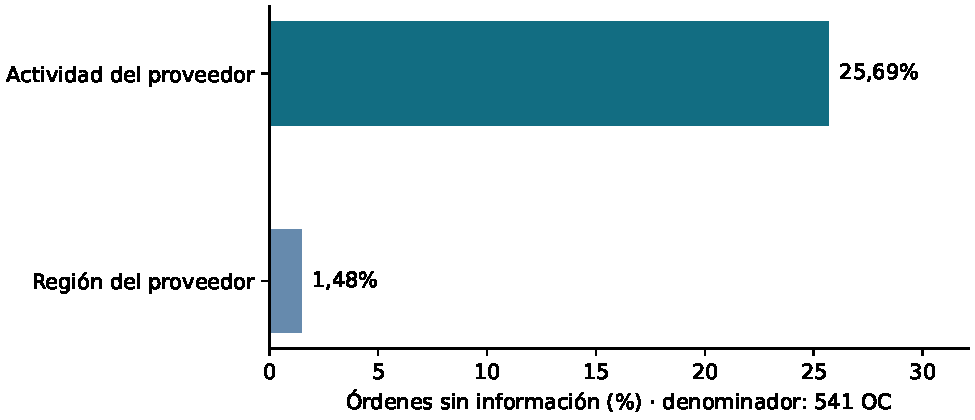
\includegraphics[width=0.95\textwidth]{figuras/faltantes_oc.pdf}
\caption{Faltantes de atributos de proveedor medidos por orden.}
\label{fig:faltantes}
{\footnotesize Nota. Elaboración mediante Matplotlib a partir de las métricas de F2.}
\end{figure}

El neto CLP tiene cero valores faltantes: no se aplica imputación por media, mediana
ni grupo. Su varianza poblacional antes y después es \VarianzaNeto{} CLP$^2$;
el cambio es cero, porque ningún importe fue reemplazado o recortado.

\subsection{Importes, fechas y valores extremos}

La conversión de números usa coma decimal y rechaza textos o formatos ambiguos.
Las fechas se interpretan explícitamente como día-mes-año. Se conservan importes y
monedas originales; la propuesta de comparación utiliza el neto CLP de la fuente.
La suma de control de las \Ordenes{} cabeceras, incluidos todos los estados, es
\NetoTotal{} CLP. No se presenta como pago efectivo ni como gasto definitivo.

La regla de Tukey marca \ExtremosNeto{} órdenes con neto CLP sobre
\UmbralNeto{} CLP. Ninguna se elimina. El mapa V2 había diagnosticado otra base:
el total de OC de las 536 órdenes CLP, con \ExtremosMapa{} extremos y umbral
\UmbralMapa{} CLP. La diferencia se explica por variable y población; ambas bases
se reproducen en el notebook. Un extremo estadístico no constituye evidencia de error.

\subsection{Vista transformada}

Se produce una tabla separada de 541 filas con:

\begin{itemize}
\item Estandarización Z del neto CLP, con media y desviación poblacional guardadas.
Una variable constante retorna cero y no divide por cero.
\item Siete columnas one-hot para las cuatro monedas y los tres estados.
Se conserva el vocabulario utilizado.
\item Tamaño ordinal Micro = 1, Pequeña = 2, Mediana = 3 y Grande = 4.
Las \TamanoDesconocido{} órdenes con NoClasificado mantienen NA e indicador.
\end{itemize}

La vista permite estudiar escalas y categorías en exploraciones posteriores, sin
modificar los importes. El ordinal expresa orden, no igualdad de distancias. La
clasificación procede del archivo y no se verificó con ventas de los proveedores.
Si se realiza modelado predictivo, los parámetros y vocabularios deberán ajustarse
solo sobre entrenamiento; esta sumativa no declara un modelo entrenado.

\section{Codificación funcional y validación}

El pipeline separa lectura, perfil, validación de cabeceras, conversiones, relaciones,
diagnóstico de detalle, transformaciones y exportación. Las funciones reciben datos
y parámetros y devuelven tablas nuevas; la exportación se concentra en una función.
El original se vuelve a verificar al finalizar.

Se ejecutaron 18 pruebas con resultado satisfactorio. Incluyen números con coma,
entrada vacía, fechas imposibles, montos contradictorios por OC, conservación de
datos, RUT con cero inicial, series constantes, categorías inesperadas y una única
categoría nominal. Las pruebas sobre el archivo real exigen conservar 541 órdenes,
las tres excepciones de detalle y las cantidades de faltantes.

Las ejecuciones locales automatizadas utilizaron un kernel nuevo por notebook.
\archivo{evidencias/ejecucion_F1.json} registra seis celdas de código ejecutadas
y cero errores; \archivo{evidencias/ejecucion_F2.json} registra doce y cero,
respectivamente. Ambos archivos identifican Windows, el motor Jupyter,
el kernel utilizado y la conservación de salidas. El resultado de las 18 pruebas
se conserva en \archivo{evidencias/pruebas_F2.json}.

Los contadores y resultados permanecen visibles en los notebooks versionados.
El flujo se detiene ante fallos. Después de exportar se recarga la tabla de órdenes;
se comprueban claves y montos con tolerancia de $10^{-7}$ CLP, compatible con los
ocho decimales exportados. Esta tolerancia numérica no tiene el mismo propósito
que el umbral de 1 CLP utilizado para el diagnóstico de conciliación.

\citet{samuel} muestran que declarar dependencias y disponer de notebooks no basta
para asegurar resultados reproducibles. En este proyecto se distinguen tres
alcances: validación asistida inicial, ejecución local en Windows y validaciones
posteriores realizadas por los integrantes del grupo en distintos equipos.
Estas comprobaciones permitieron contrastar la ejecución del proyecto entre
Windows 10 y Windows 11, utilizando Python 3.13.15 en las validaciones locales
posteriores a la comprobación inicial.

\section{Control de versiones y trazabilidad}

El historial Git revisado permite identificar contribuciones sustantivas de
los cuatro integrantes del grupo. Para esta síntesis se consideran commits
representativos de implementación, validación, documentación técnica y
trazabilidad, excluyendo cambios correspondientes únicamente a bitácoras y
commits de merge.

\begin{table}[H]
\centering
\small
\begin{tabular}{p{2.7cm} p{2.0cm} p{8.0cm}}
\toprule
Integrante & Commit & Contribución representativa \\
\midrule
mín Araya & \texttt{9b266b2} & Crea la estructura inicial del proyecto. \\
& \texttt{0a132d4} & Agrega el mapa conceptual corregido según retroalimentación docente. \\
& \texttt{8b4fcb6} & Incorpora la base asistida para revisión del grupo. \\
& \texttt{6632bd9} & Registra ejecución local de F1 en Windows. \\
& \texttt{5a4325e} & Registra validación local y resultados de F2. \\
\midrule
Alan Cañete & \texttt{fd1e8d0} & Incorpora el dataset utilizado en el proyecto. \\
& \texttt{122bb02} & Ajusta el tratamiento de la excepción del CSV para incorporar el dataset. \\
\midrule
Jorge Guaico & \texttt{009b81d7} & Registra validación local de Jorge en Windows. \\
\midrule
Patricio Cortez & \texttt{ceb01fe} & Valida el entorno Python 3.13 y las dependencias de F2. \\
& \texttt{aa39e91} & Registra la validación de ejecución reproducible de F2. \\
& \texttt{5be9729} & Registra la ejecución del pipeline de F2. \\
& \texttt{621d816} & Valida las pruebas automatizadas de F2. \\
& \texttt{919e9c1} & Registra la validación completa de ejecución de F1 y F2. \\
\bottomrule
\end{tabular}
\caption{Contribuciones representativas identificadas en el historial Git.}
\label{tab:contribuciones_git}
\end{table}

La tabla no pretende representar la totalidad del trabajo realizado por cada
integrante, sino evidenciar mediante el historial versionado distintas
contribuciones técnicas y de validación realizadas durante el desarrollo.


La ejecución de F1 actualizada quedó incorporada en \archivo{45ea1ad}, y la de
F2 en \archivo{5a4325e}. El campo \archivo{revision_git_al_ejecutar} de cada
evidencia corresponde al commit presente al iniciar esa ejecución, que precede
al commit que guarda sus resultados. La huella de la fuente del notebook se
registra por separado; no se reemplaza aquel identificador por uno posterior.

Los avances documentados acreditan contribuciones individuales de los cuatro
integrantes del grupo mediante el historial Git y la bitácora. Benjamín
registró la estructura inicial y las primeras validaciones; Alan incorporó y
ajustó el tratamiento del dataset; Jorge registró su validación local; y
Patricio documentó validaciones de entorno, ejecución reproducible, pipeline,
pruebas automatizadas y ejecución completa de F1 y F2. La revisión colectiva
de las decisiones y evidencias forma parte de la preparación final del
informe.

Se retiró el filtro local de nbstripout y se verificó el contenido preparado para
los commits mediante \archivo{scripts/verificar_entrega.py} con la opción
\texttt{-{}-staged}. Esta revisión
comprobó la presencia de celdas ejecutadas y salidas; no certifica por sí sola la
corrección metodológica ni la calificación del equipo.

El código, los notebooks con resultados, la documentación y las evidencias de
validación se encuentran publicados en la rama de trabajo. El original y las
tablas individuales se mantienen como insumos de trabajo y su tratamiento se
documenta mediante los archivos y evidencias disponibles en el repositorio.
Las dependencias fueron instaladas y comprobadas en el entorno local utilizado
para la validación final, y la ejecución de F1 y F2 fue contrastada en equipos
con Windows 10 y Windows 11. El entorno virtual y los auxiliares de compilación
no se versionan.

\clearpage
\section{Vinculación con el mapa conceptual V2}

El mapa corregido se mantiene como documento legible en
\archivo{F1/docs/Mapa_conceptual_Grupo7_V2.pdf}, junto a su editable. La tabla
\ref{tab:mapa} vincula sus conceptos con evidencias; la correspondencia completa
está en \archivo{docs/vinculacion_mapa.md}.

\begin{table}[H]
\caption{Conceptos implementados y trabajo proyectado}
\label{tab:mapa}
\small\singlespacing
\begin{tabularx}{\textwidth}{@{}>{\raggedright\arraybackslash}p{0.24\textwidth}>{\raggedright\arraybackslash}p{0.34\textwidth}Y@{}}
\toprule
Concepto & Estado & Evidencia\\
\midrule
Definición y entorno & Ejecutado y validado en Windows & Notebook F1, configuración y evidencias de ejecución.\\
Adquisición y raw & Lectura y trazabilidad documentadas; acceso compartido según disponibilidad de los insumos & F1/data/raw y manifiesto.\\
Exploración & Implementada y validada & Notebook F2, secciones 2 y 3.\\
Limpieza y transformación & Implementadas y validadas & F2/src, parámetros exportados y evidencias del pipeline.\\
Git versiona la limpieza & Código, resultados, documentación y aportes técnicos versionados & Commits de la tabla \ref{tab:commits} y bitácora.\\
Jupyter documenta exploración & Implementado con salidas conservadas & Notebooks ejecutados y evidencias de ejecución.\\
Rubros & Pertenencia implementada; asignación de montos por rubro mantiene excepciones identificadas & Puente, métricas y excepciones de detalle.\\
Visualización y reporte & Figura diagnóstica e informe LaTeX en desarrollo & Matplotlib, LaTeX y script de compilación.\\
F3 y F4 & Proyectadas & Sin declarar ejecución ni entregables futuros cerrados.\\
\bottomrule
\end{tabularx}
\end{table}


\clearpage
\section{Reflexión técnica y próximos pasos}

La decisión central es separar las unidades presentes en el archivo. Validar
atributos de cabecera permite obtener una tabla de órdenes sin multiplicar sus
importes. Sin embargo, la conciliación de firmas no resuelve todas las multiplicidades
del detalle. Esta limitación impide asignar montos por rubro con la evidencia actual,
aunque sí permite conservar y estudiar relaciones de pertenencia.

Las alternativas descartadas tienen consecuencias observables: eliminar por
actividad perdería 139 órdenes; imputar la moda asignaría información desconocida;
deduplicar el detalle de la OC 264 quitaría un millón de CLP. Conservar datos y
declarar excepciones produce una base más defendible que presentar esas decisiones
como automáticamente resueltas.

Antes de entregar se deben realizar las siguientes revisiones finales:

\begin{enumerate}
\item Revisar la definición de montos, la conversión a CLP y el tratamiento
documentado de las tres excepciones de detalle.
\item Revisar la justificación del filtro de estados y las transformaciones
aplicadas en la bitácora.
\item Verificar que la documentación de procedencia del original incluya la
URL y fecha de descarga, cuando corresponda.
\item Revisar la consistencia entre las dependencias documentadas, los
entornos utilizados y las evidencias de ejecución.
\item Revisar la correspondencia entre los aportes y validaciones de los cuatro
integrantes y el historial Git.
\item Revisar la versión final del informe, sus metadatos y las evidencias
antes de la entrega.
\end{enumerate}



\clearpage
% Referencias autor-fecha y formato APA 7; orden alfabético y sangría francesa.
% Los materiales docentes adjuntos no incluyen autor o fecha explícitos.
% Confirmar metadatos con el curso antes de la entrega; no inventarlos.
\begin{thebibliography}{}

\bibitem[{\emph{Guía de desarrollo}}(s. f.)]{guia}
\emph{Guía de desarrollo: Evaluación Sumativa 1 (Fases 1 y 2)}. (s. f.).
[Documento de apoyo de la asignatura MCDI500 facilitado al equipo].

\bibitem[NumPy Developers(s. f.)]{numpy}
NumPy Developers. (s. f.). \emph{numpy.percentile}. NumPy documentation.
Recuperado el 13 de septiembre de 2026, de
\url{https://numpy.org/doc/stable/reference/generated/numpy.percentile.html}

\bibitem[pandas Development Team(s. f.)]{pandas}
pandas Development Team. (s. f.). \emph{pandas.read\_csv}. pandas documentation.
Recuperado el 13 de septiembre de 2026, de
\url{https://pandas.pydata.org/docs/reference/api/pandas.read_csv.html}

\bibitem[Project Jupyter(s. f.)]{jupyter}
Project Jupyter. (s. f.). \emph{File and output formats}. JupyterLab documentation.
Recuperado el 13 de septiembre de 2026, de
\url{https://jupyterlab.readthedocs.io/en/stable/user/file_formats.html}

\bibitem[{\emph{Rúbrica sumativa 1}}(s. f.)]{rubrica}
\emph{Rúbrica sumativa 1 fase 1 y 2}. (s. f.).
[Rúbrica de evaluación de la asignatura MCDI500 facilitada al equipo].

\bibitem[Samuel y Mietchen(2023)]{samuel}
Samuel, S., \& Mietchen, D. (2023).
\emph{Computational reproducibility of Jupyter notebooks from biomedical publications}
[Prepublicación]. arXiv.
\url{https://doi.org/10.48550/arXiv.2308.07333}

\bibitem[Peng(2011)]{peng2011}
Peng, R. D. (2011).
Reproducible research in computational science.
\emph{Science}, 334(6060), 1226--1227.
\url{https://doi.org/10.1126/science.1213847}

\bibitem[Sandve et al.(2013)]{sandve2013}
Sandve, G. K., Nekrutenko, A., Taylor, J., \& Hovig, E. (2013).
Ten simple rules for reproducible computational research.
\emph{PLoS Computational Biology}, 9(10), e1003285.
\url{https://doi.org/10.1371/journal.pcbi.1003285}

\end{thebibliography}


\end{document}
